\documentclass[iop,twocolumn]{emulateapj}
\pagestyle{myheadings}
%\usepackage{bm}
%\usepackage{amsfonts}
%\usepackage{enumerate}
\usepackage{amsmath}
\usepackage{placeins}
\usepackage{graphics}
\usepackage{color}
\usepackage{braket}
\usepackage{amssymb}
\usepackage{hyperref}
\shorttitle{HW6}
\shortauthors{Jensen}

\newcommand{\Ham}{\mathcal{H}}
\newcommand{\deriv}[2]{\frac{\textrm{d} #1}{\textrm{d} #2}}
\newcommand{\p}[2]{\frac{\partial #1}{\partial #2}}
\begin{document}

\title{Term Project 1D MHD}

\author{
Trey~W.~Jensen\altaffilmark{1}
}

\altaffiltext{1}{
Department of Physics,
New York University, New York, NY 10003, USA
}
\date{\today}

\email{TJ796@nyu.edu}

\section{Magnetohydrodynamics}\label{sec:MHD}
Magnetohydrodynamics (MHD) is an extension of hydrodynamics, where, on top of normal fluid equations such as the continuity equation and Euler equation, electromagnetism is added as if threading each fluid element. The partial differential equation we solve is of the general elliptic form,
\begin{equation}
  \p{{\bm U} {\bm  U}}{t}+\p{{\bm F}}{x}=0 \label{eq:1},
\end{equation}
where ${\bm U}$ is a vector of conserved quantities, and ${\bm F}$ is the vector of fluxes of those conserved quantities. In an adiabatic one-dimensional hydrodynamic code, we have inital conserved quantities mass, momentum, and energy written as ${\bm U}=(\rho,\rho v,E)^T$, where $\rho$ is the density, $v$ the one-dimensional velocity, and $E$ is the energy (transpose to signify it as a vector quantity). We compute $E$ through $E=\rho e + \frac{1}{2}\rho v^2$, where the specific internal energy is found through the equation of state $P=(\gamma-1)\rho e$ (where $\gamma$ is the adiabatic index of our ``ideal'' fluid). The three conserved quantities, $\rho,\,\rho v,\,E$, have fluxes given by ${\bm F}=(\rho v,\rho v^2+P,(E+P)v)^T$.
If we want to simulate charged particles (or fluids) we are neglecting all the possible electromagnetic contributions. To account for this, we utilize the differential forms of Maxwell's equations and Amp{\`e}re's law, and substituting Ohm's law and Lorentz force to replace terms of the electric field (with ideal approximations). More explicitly we solve the equations (following closely from \cite{stone08a}; units are such that the magnetic permeability $\mu=1$),
\begin{align*}
  \p{\rho}{t}+\nabla\cdot(\rho{\bm v})&=0,\quad\textrm{(mass cons.)}\\
  \p{\rho{\bm v}}{t}+\nabla\cdot\left(\rho{\bm v}{\bm v}-{\bm B}{\bm B}+P^*\right)&=0,\quad\textrm{(momentum cons.)}\\
  \p{E}{t}+\nabla\cdot\left((E+P^*){\bm v}-{\bm B}({\bm B}\cdot v)\right)&=0,\quad\textrm{(energy cons.)}\\
  \p{{\bm B}}{t}-\nabla\times({\bm v}\times{\bm B})&=0,\quad\textrm{(Maxwell's eq.)}
\end{align*}
where, in the case of one-dimension MHD, we have the conserved quantities and fluxes given by,
\begin{align*}
  {\bm U}=
  \begin{bmatrix}
    \rho \\
    v_x\\
    v_y\\
    v_z\\
    P\\
    B_x\\
    B_y\\
    B_z\\
  \end{bmatrix}
  ,\quad {\bm F}=
  \begin{bmatrix}
    \rho v_x \\
    \rho v_x^2+P+B^2/2-B_x^2\\
    \rho v_xv_y-B_xB_y\\
    \rho v_xv_z-B_xB_z\\
    (E+P^*)v_x-({\bm B}\cdot{\bm v})B_x\\
    0\\
    B_yv_x-B_xv_y\\
    B_zv_x-B_xv_z\\
  \end{bmatrix},
\end{align*}
where $B$ is the magnetic field, $P^*=P+B^2/2$ is the total pressure, and here the total energy density is given by,
\begin{equation*}
  E=\frac{P}{\gamma-1}+\frac{1}{2}\rho v^2+\frac{B^2}{2}.
\end{equation*}
These are very similar to the plain hydrodynamics version, but just some added terms such as pressure generated from the magnetic field, the energy stored in it, and the evolution of the magnetic field due the flow of particles. There is no evolution of $B_x$ due to the derivation of these fluxes leading to a $B_xv_x-B_xv_x$ term that goes to zero when the dimension being considered is in the $x$-direction. An important criterion for physical results is for the divergence of the magnetic field to be zero, $\nabla\cdot B=0$. We see that the flux/change in $B_y$ and $B_z$ are curls that by design go to zero when taking the divergence. As long as we have a constant $B_x$ field, we will satisfy the criterion. Taking this to more dimensions complicates the situation, and other methods are required to ensure physical reality (see \cite{stone08a}).
\subsection{Computational Methods}
To solve for the MHD equations in Section~\ref{sec:MHD} requires solving for both a time step and spacial step. For the time progression, we implement a third-order Runge-Kutta scheme combined with forward Euler, given by,
\begin{align*}
  {\bm U}^{(1)}&={\bm U}^n+\Delta t L({\bm U}^n),\\
  {\bm U}^{(2)}&=\frac{3}{4}{\bm U}^n+\frac{1}{4}{\bm U}^{(1)}+\frac{1}{4}\Delta t L({\bm U}^{(1)}),\\
  {\bm U}^{n+1}&=\frac{1}{3}{\bm U}^n+\frac{2}{3}{\bm U}^{(2)}+\frac{2}{3}\Delta t L({\bm U}^{(2)}),
\end{align*}
where $n$ signifies the $n$-th time step, and $L(U)$ is given by,
\begin{align*}
  L(U)=-\frac{{\bm F}_{i+1/2}-{\bm F}_{i-1/2}}{\Delta x}.
\end{align*}
We discretize our fluid into spacial cells that receive flux from the neighboring cells. We center our coordinates in the center of these cells, thus $i+1/2$ ($i-1/2$) would be the right (left) interface of the $i$-th cell. There are discontinuties at each interface (obviously from the discretization) that require a Riemann solver. In this case we use the Harten, Lax, van Leer (HLL) Riemann solver given by,
\begin{align*}
  {\bm F}^{HLL}=\frac{\alpha^+{\bm F}^L+\alpha^-{\bm F}^R-\alpha^+\alpha^-({\bm U}^R-{\bm U}^L)}{\alpha^++\alpha^-},
\end{align*}
where $\alpha^\pm$ are found from the minimal and maximal eigenvalues, $\lambda$, of the Jacobian of the conserved variables,
\begin{align*}
  \lambda=(v_x-C_f,v_x-C_A,v_x-C_s,v_x+C_s,v_x+C_A,v_x+C_f)
\end{align*}
where $C_{f,s}$ are the fast and slow-magnetosonic wave speeds and $C_A$ is the Alfv{\'e}n wave speed (see \cite{stone08a} for more details), given by,
\begin{align*}
  C_{f,s}^2&=\frac{1}{2}\left(c^2+b^2\pm\sqrt{(c^2+b^2)^2-4c^2b_x^2}\right),\\
  C_A^2&=\frac{B_x^2}{\rho},
\end{align*}
where,
\begin{align*}
  b^2&=\frac{B^2}{\rho},\\
  b_x^2&=\frac{B_x^2}{\rho},\\
  c^2&=\frac{\gamma P}{\rho}.
\end{align*}
These are the waves of ``information'' travel, and thus taking the fastest wave in both direction (minimal and maximal) will be the interface of which we want our Riemann solver to address.
For a higher-order method of space, we compute the slopes of the quantities {\it near} the interfaces and feed them into $F^{HLL}$, which feeds into $L(U)$. For example,  the left side of the right interface of the $i$-th cell is found via,
\begin{align*}
  &c^L_{i+1/2}= c_i +\frac{1}{2} \\
  &\quad\times\textrm{minmod}\left(1.5(c_i-c_{i-1}),0.5(c_{i+1}-c_{i-1}),1.5(c_{i+1}-c_i)\right),
\end{align*}
where $c$ is the input inital condition parameters (or, namely, conserved quantities), and the function minmod, defined by,
\begin{align*}
  \textrm{minmod}(x,y,z)&=\quad\frac{1}{4}|\textrm{sgn}(x)+\textrm{sgn}(y)|\\
  &\quad\times(\textrm{sgn}(x)+\textrm{sgn}(z))\textrm{min}(|x|,|y|,|z|),
\end{align*}
where sgn is the sign of the input, ensures that we do not accidentally ``overshoot'' the approximation causing inaccurate quantity differentials. We can see that this requires two neighboring cells on either side of the computed interface, implying that we need two {\it ghost} cells on the left for the first cell, and on the right for the last cell. We use a Dirichlet boundary condition, where we simply fix the {\it ghost} cells as the initial conditions. Ultimately, using these newly computed conserved quantities from the higher-order spacial scheme ensures our interface flux is more accurately represented.
\section{Validity and Execution}
A famous test is the Brio $\&$ Wu MHD Shock Tube Test problem. The initial conditions are step functions centered at $x_0=0.5$ with,
\begin{align}\label{eq:ic}
  \begin{bmatrix}
    \rho \\
    v_x\\
    v_y\\
    v_z\\
    P\\
    B_x\\
    B_y\\
    B_z\\
  \end{bmatrix}
  \textrm{(Left)}=
  \begin{bmatrix}
    1\\
    0\\
    0\\
    0\\
    1\\
    0.75\\
    1\\
    0\\
  \end{bmatrix}
  ,\quad\&\quad
  \begin{bmatrix}
    \rho \\
    v_x\\
    v_y\\
    v_z\\
    P\\
    B_x\\
    B_y\\
    B_z\\
  \end{bmatrix}
  \textrm{(Right)}=
  \begin{bmatrix}
    0.125\\
    0\\
    0\\
    0\\
    0.1\\
    0.75\\
    -1\\
    0\\
  \end{bmatrix},
\end{align}
and $\gamma=2$. The results of running these initial conditions to $t_f=0.12$ are shown in Figure~\ref{fig:f1}, and qualitatively agree well with what is in the literature (see \url{https://astro.uni-bonn.de/~jmackey/jmac/node7.html} for example). This test reveals proper propagation of waves, including the compound waves, rarefactions, contact discontinuities, and shocks. For a more quantitative approach of validity, we introduce isentropic initial conditions that, by physical design, maintain entropy. The initial conditions were given by,
\begin{align}
  \rho(x)&=\rho_0(1+\alpha f(x))\nonumber\\
  P(x)&=P_0\left(\frac{\rho(x)}{\rho_0}\right)^\gamma\nonumber\\
  B_y(x)&=(1+\alpha f(x))\label{eq:icis}
\end{align}
\begin{figure*}[htb!]
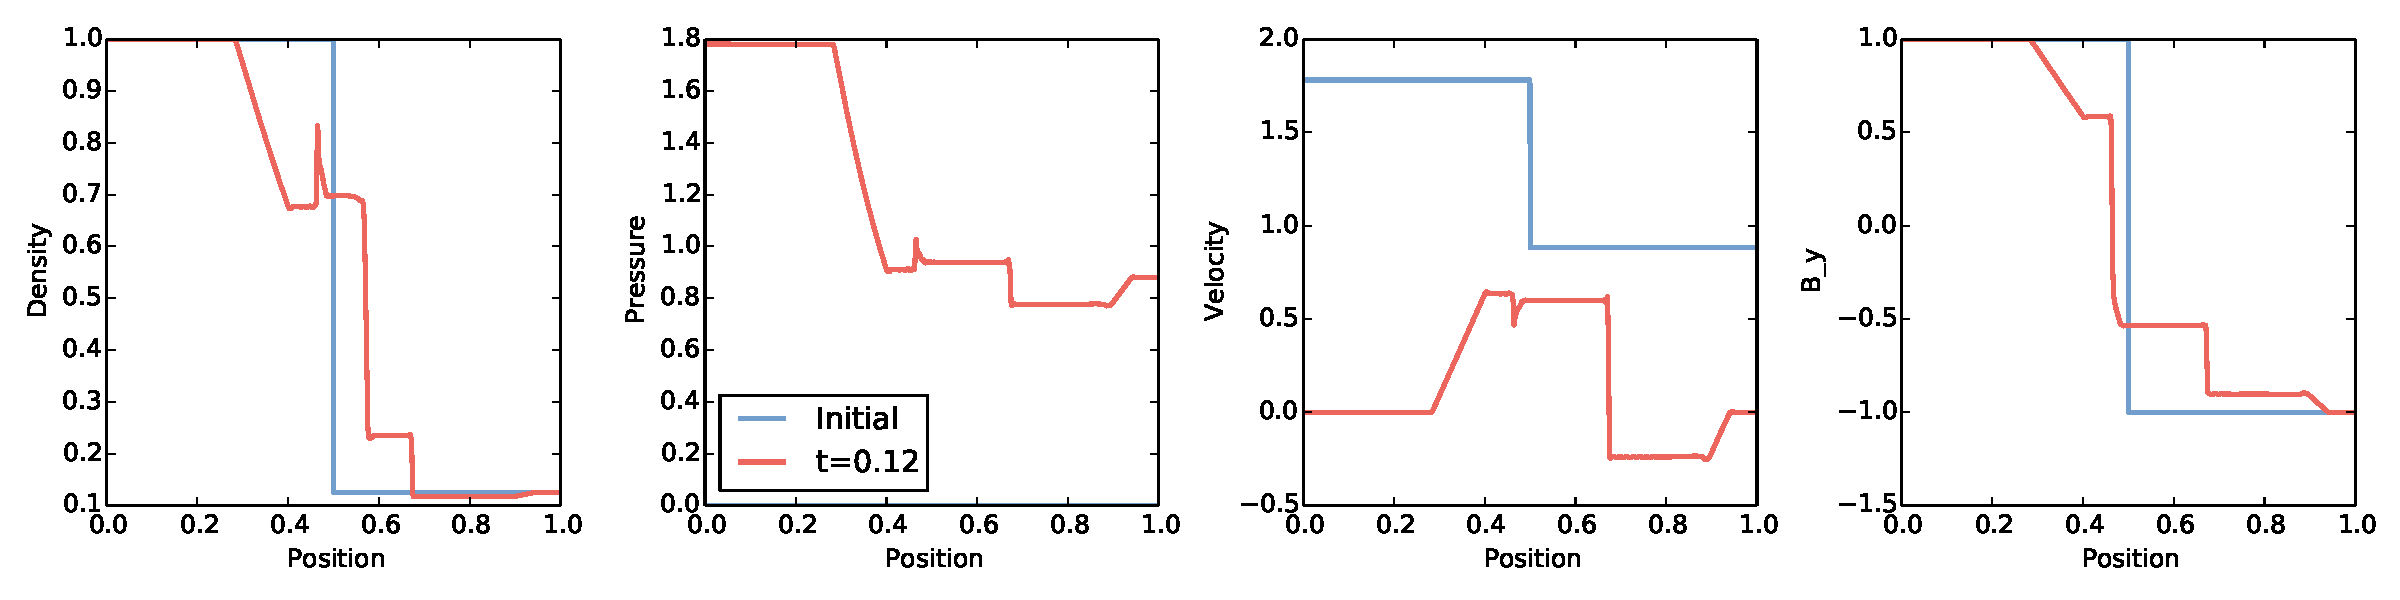
\includegraphics[scale=.45,trim=0cm 0cm 0cm 0cm,clip]{f1.pdf}
\caption{Plot of the density, pressure, velocity in the $x$-direction, and magnetic field in the $y$-direction. The initial conditions are given in Eq.~\ref{eq:ic}. The simulation ran until $t=.12$. This is for $N=1000$ spacial grid cells. The units are arbitrary. \label{fig:f1}}
\end{figure*}
where $\rho_0=1$,$P_0=1$, $\alpha=0.2$, $\gamma=5/3$, and $f(x)$ is a 1-$\sigma$ gaussian perturbation centered on $x_0=2$ with $\sigma=0.4$, where everything outside of $|x-x_0|<\sigma$ is zero. We can see the outcome of the simulation at $t_f=1$ (and intermediate intervals) in Figures~\ref{fig:f3}~\&~\ref{fig:f2}. To check if our simulation obeys theoretical physical prediction, we computed how the integrated $L_1$ error in entropy (i.e. $|s_0-s_f|$) scales with the number of steps $N$. We see a slope of convergence $L_1\propto N^m$ with $m\approx-2.57$ which implies this was higher than a second-order result. This problem is well-behaved for short time periods with no discontinuities or jumps, so convergence is also well-behaved. Finally, we tested the consequences of perturbing a uniform, equilibrium fluid with a gaussian magnetic field ($B_y$ identical to that in Eq.~\ref{eq:icis}). Here we generated a movie that can be seen at \url{https://youtu.be/JJbPpWo2wpA}. This simulation ultimately reveals the consequences of Alfv{\'e}n waves. The initial magnetic field in the $y$ direction wants to repel, and initially splits into two Alfv{\'e}n waves, but in order to do this, it drags the material with it leaving a void of density at the inital perturbation. This void would normally be filled in, but because of the magnetic field also battling movement of fluid, it creates a self-sustained void in pressure and density, trapping the surplus magnetic field at the center. The two Alfv{\'e}n waves propagate indefinitely dragging fluid with it.
\begin{figure}[htb!]
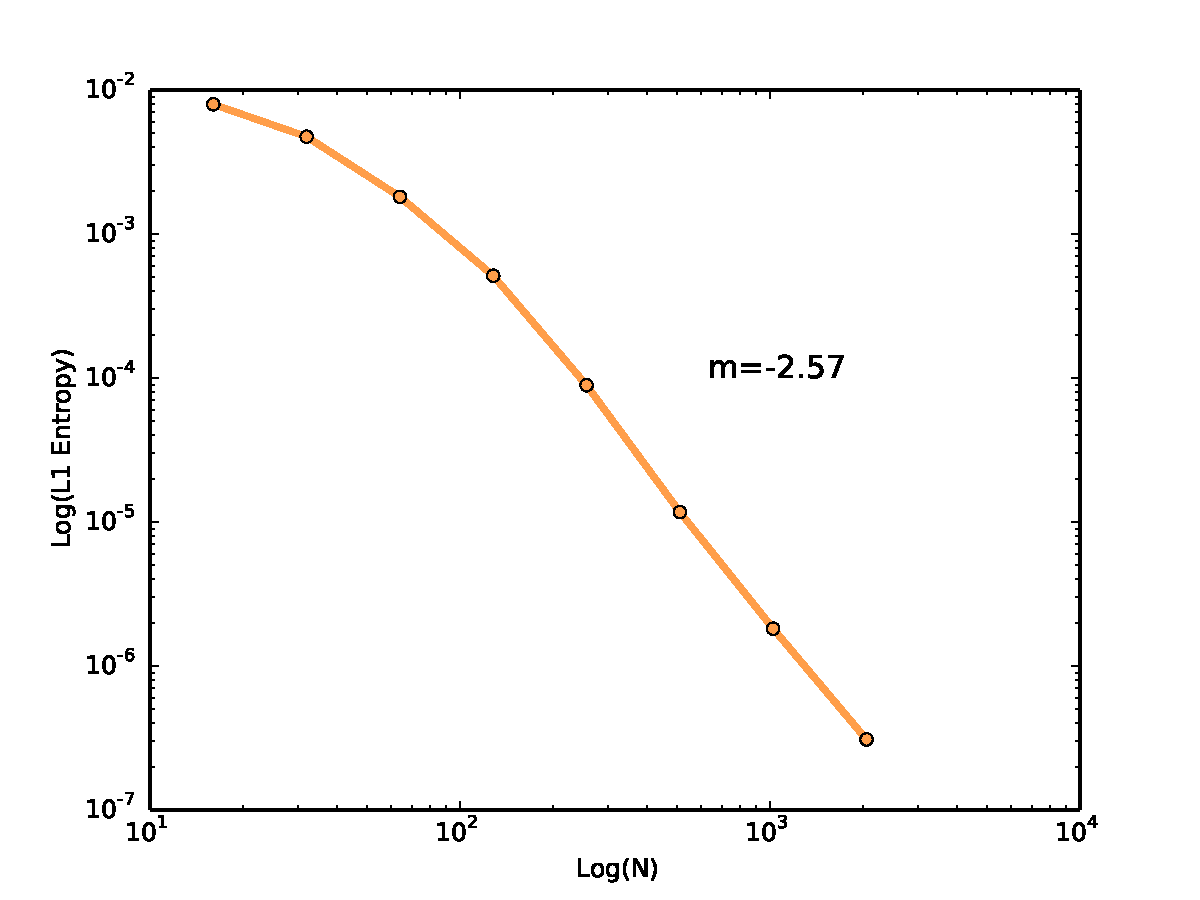
\includegraphics[scale=.45,trim=0cm 0cm 0cm 0cm,clip]{f3.pdf}
\caption{Log-Log plot of the convergence of iterating the simulation of initial conditions given by Eq.~\ref{eq:icis} with different number of spacial grid cells, $N$. The slope of convergence, $m$, is reported. \label{fig:f3}}
\end{figure}
\section{Future Work}
The original inspiration for this work was to model the galactic magnetic field of the Milky Way galaxy. Unfortunately that requires a three-dimensional algorithm and is the scale of a Ph.D. thesis. More specifically, the next steps would be to try to extend this to spherical coordinates and impose sheering velocities from the gravitational potential such as a black hole, to ultimately, given an initial magnetic field of poloidal geometry, see how this initial field alters. Along with this, implementing striated random fields within the disk to mimic super novae within the galaxy or the like as mentioned in \cite{jansson12a}. These goals require a supercomputer, and are, of course, over-ambitious in nature for a project such as this.\\
\vspace{1.2cm}
\\
I would like to thank Professor MacFadyen for the intricate and well organized lectures that gave way to even learning Python from scratch, and supplied resources to dabble near the frontier of research regarding computational physics. And especially to Geoff, who put up with an impossible amount of shit from all students, me included. I would go postal having to pore through amateurish (again, I am not excluded) programs. Thank you.

\begin{figure*}[htb!]
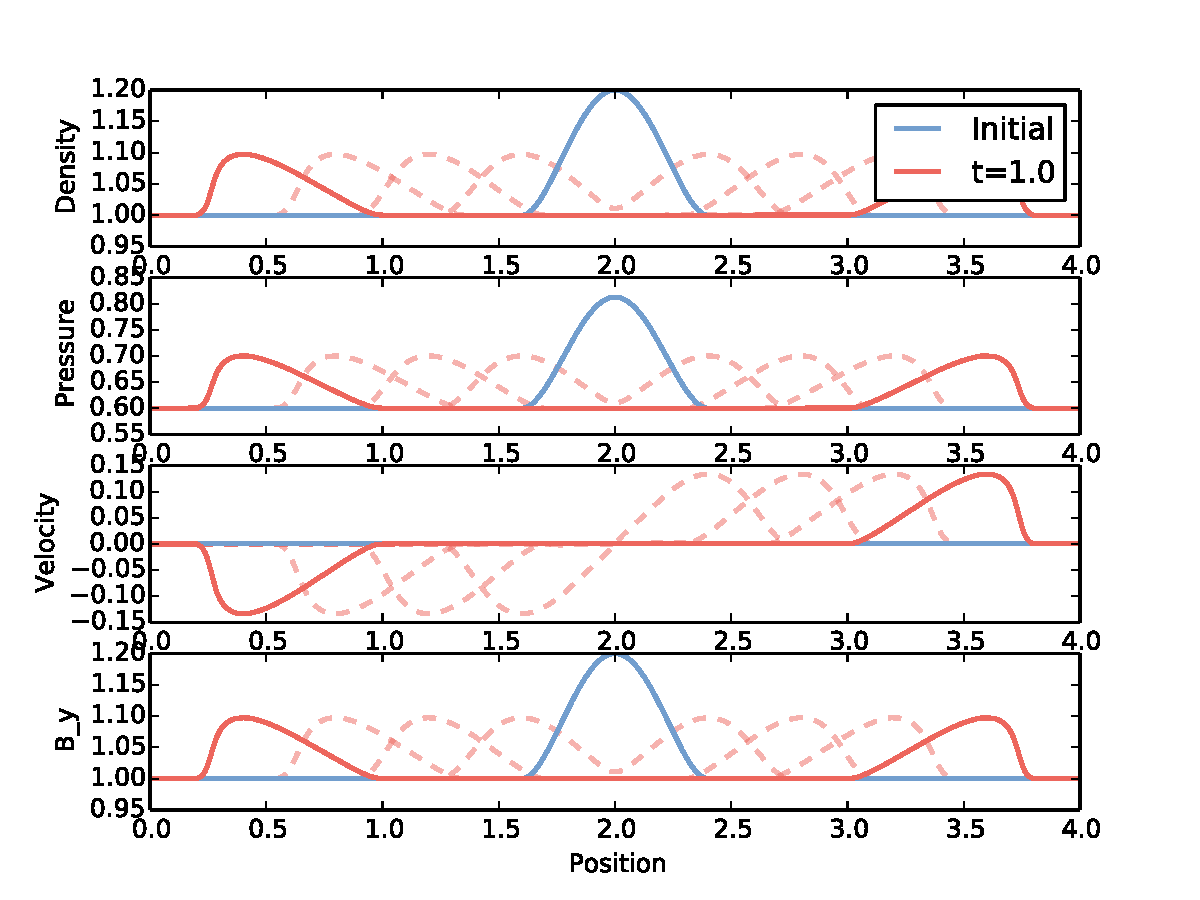
\includegraphics[scale=.9,trim=0cm 0cm 0cm 0cm,clip]{f2.pdf}
\caption{Plot of the density, pressure, velocity in the $x$-direction, and magnetic field in the $y$-direction. The inital conditions are given in Eq.~\ref{eq:icis}. The semitransparent lines are intermediate time steps. This is for $N=1000$ spacial grid cells. The units are arbirtary. \label{fig:f2}}
\end{figure*}
\bibliographystyle{mnras}
\bibliography{bibliography}
\end{document}
